\documentclass{beamer}

\usepackage[utf8]{inputenc}
\usepackage[ngerman]{babel}
\usepackage{beamerthemeshadow}
\usepackage{calc}
\usepackage{ifthen}
\usepackage{tikz}
\usepackage{caption}
\usepackage{subcaption}
\usepackage{bchart}
\usepackage{wrapfig}
\usepackage{ulem}
\usepackage{color}
\usepackage{epigraph}
\usepackage{tipa}

\definecolor{darkgreen}{rgb}{0.2,0.6,0.2}

\usepackage{listings}

\title{Kollaborative Textverarbeitung}
\subtitle{mit \LaTeX, Git und Github}
\author{Ervin Mazlagic}
\institute{Zentralschweizer OpenSource Verein \\\textbf{LuXeria}}

\begin{document}
\maketitle

% Listing settings
\lstset{
%    morekeywords={\tableofcontents},
    breakwhitespace=true,
    language=[LaTeX]TeX,
    basicstyle=\footnotesize\ttfamily,
    keywordstyle=\color{red}\bfseries,
    idnetifierstyle=\color{blue},
    commentstyle=\color{darkgreen},
    stringstyle=\color{blue},
    columns=fullflexible,
    keepspaces=true,
    breaklines=true,
    tabsize=3,
    showstringspaces=false,
    extendedchars=true,
    literate={Ö}{{\"O}}1
    	     {ö}{{\"o}}1
	     {Ä}{{\"A}}1
	     {ä}{{\"a}}1
	     {Ü}{{\"U}}1
	     {ü}{{\"u}}1,
    morekeywords={
	\begin, 
	\item,
	\end,
	\tableofcontents}
}

\section{Einleitung}

\subsection{Person}
\begin{frame}
	\frametitle{Wer bin ich? \hfill{} \footnotesize{LuXeria}}
	\begin{block}{Personalien, Ausbildung \& Hobby}
		\begin{itemize}
			\item Ervin Mazlagic
			\item Perlen (LU), Biha\'c (BiH)
			\item Student ET, HSLU-T\&A
			\item Elektroniker - R\&D
			\item Schindler Aufzüge AG, FU-HW-Entwicklung
			\item Präsident des LuXeria
		\end{itemize}
	\end{block}
\end{frame}

\subsection{Ziele}
\begin{frame}
	\frametitle{Was soll erreicht werden? \hfill{} \footnotesize{LuXeria}}
	\begin{block}{Nach dieser Präsentation können Sie}
		\begin{itemize}
			\item WYSIWYG von \TeX~\& \LaTeX~unterscheiden
			\item Git und seine Eigenschaften nennen
			\item Funktionen und Philisophie von Github nennen
			\item Einsatz von \LaTeX, Git und Github abschätzen
			\item selbstständig weitere Informationen finden
		\end{itemize}
	\end{block}
\end{frame}

\subsection{Zielgruppen}
\begin{frame}
	\frametitle{An wen richtet sich diese Präsentation? \hfill{} \footnotesize{LuXeria}}
	\begin{exampleblock}{An jene die}
		\begin{itemize}
			\item Texte aller Art zusammen erstellen/bearbeiten wollen
			\item Texte mit Projektmanagement verwalten möchten
			\item \LaTeX, Git und Github nicht kennen/gewohnt sind
			\item eine Alternative zu kollaborativem Texten suchen
		\end{itemize}
	\end{exampleblock}

	\begin{alertblock}{Nicht an jene die}
		\begin{itemize}
			\item Git und Github bereits kollaborativ benutzen
			\item auf MS-Office-Formate nicht verzichten können
		\end{itemize}
	\end{alertblock}
\end{frame}

\subsection{Programm}
\begin{frame}
\frametitle{Programmübersicht \hfill{} \footnotesize{LuXeria}}
	\tableofcontents[hideallsubsections]
\end{frame}

\section{\TeX~\& \LaTeX}
\begin{frame}
	\frametitle{}
	\tableofcontents[currentsection]
\end{frame}

\subsection{WYSIWYG und Andere}
\begin{frame}
	\frametitle{What You See Is What You Get? \hfill{} \footnotesize{LuXeria}}
	\begin{columns}
		\begin{column}{5cm}
			\begin{alertblock}{WYSIWYG}
				\begin{itemize}
					\item Was du siehst ist das, was du bekommst!
					\item Interagiert mit Systemdaten (Druckertreiber etc.)
					\item unvorhersagbar
					\item undruchsichtig
					\item Bsp. MS-Office
				\end{itemize}
			\end{alertblock}
		\end{column}
		\begin{column}{5cm}
			\begin{exampleblock}{\TeX~\& \LaTeX}
				\begin{itemize}
					\item Was du bekommst ist das, wonach du gefragt hast!
					\item System- und Plattformunabhängig
					\item vorhersagbar (Programm)
					\item Frei (free speech \& free beer)
					\item professioneller Satz
				\end{itemize}
			\end{exampleblock}
		\end{column}
	\end{columns}
\end{frame}

\subsection{\LaTeX}
\begin{frame}[fragile]
	\frametitle{\LaTeX \hfill{} \footnotesize{LuXeria}}
	\framesubtitle{Aufbau von \TeX-Dokumenten}
	\begin{block}{Präambel}
	Hier stehen Definitionen zu Layout und Funktionalität.
	\end{block}
	\begin{block}{Dokumenteninhalt}
	Hier steht der Inhalt als 'reiner' Inhalt.
		\begin{columns}
			\begin{column}{6cm}
				\begin{alertblock}{externe Inhalte}
					Externe Inhalte die eingebunden werden wie Bilder, Verzeichnisse etc.
				\end{alertblock}
			\end{column}
		\end{columns}
	\end{block}
\end{frame}


\begin{frame}[fragile]
	\frametitle{\LaTeX \hfill{} \footnotesize{LuXeria}}
	\framesubtitle{Immer \& überall das selbe Ergebnis!}
	\begin{columns}
		\begin{column}{5cm}
			\begin{block}{\LaTeX~Code}
				
\begin{lstlisting}{Bsp}
Einige Vorteile von \LaTeX:

% Hier folgt 
% eine Aufzaehlung
\begin{itemize}
  \item Freie Software
  \item $\sum\frac{n}{1-n^2}$
  \item Professioneller Satz
\end{itemize}
\end{lstlisting}
				
			\end{block}
		\end{column}
		\begin{column}{5cm}
			\begin{block}{Ausgabe}
				Einige Vorteile von \LaTeX:
				% eine Aufzaehlung
				\begin{itemize}
					\item Freie Software
					\item $\sum\frac{n}{1-n^2}$
					\item Professioneller Satz
				\end{itemize}
			\end{block}
		\end{column}
	\end{columns}
\end{frame}

\section{Git \& Github}
\begin{frame}
	\frametitle{}
	\tableofcontents[currentsection]
\end{frame}

\subsection{Git}
\begin{frame}
	\frametitle{Git --- Dummkopf \hfill{} LuXeria}
	\framesubtitle{Was ist Git?}
	\begin{columns}
		\begin{column}{5cm}
			\begin{figure}
				
\includegraphics[width=0.8\columnwidth]{git_logo.pdf}
				\caption{neues Git-Logo}
			\end{figure}
			\footnotesize{
			\textbf{git}[\textipa{git}] - a bastard or fool
			\epigraph{ I'm an egoistical bastard, and I name all my projects after myself.
				First Linux, now git.}{Linus Torvalds}
			}\normalsize
		\end{column}
		\begin{column}{5cm}
			\begin{block}{Überblick}
				\begin{itemize}
					\item Verwaltungssystem
					\item nicht linear
					\item dezentral
					\item sicher \& stabil
					\item OpenSource
					\item Plattformunabhängig
				\end{itemize}
			\end{block}
		\end{column}
	\end{columns}
\end{frame}

\begin{frame}
	\frametitle{Git --- nicht linear?\hfill{} LuXeria}
	\framesubtitle{Arbeiten mit Forks und Branches}
	\begin{columns}
		\begin{column}{5cm}
			\begin{figure}
				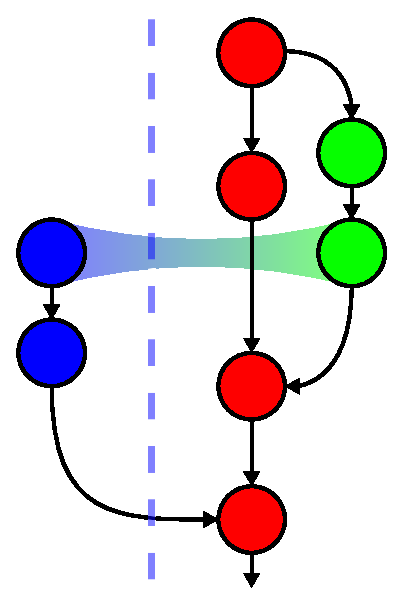
\includegraphics[scale=0.5]{git_tree.eps}\\
				\textcolor{blue}{Fork} -- \textcolor{red}{master} -- \textcolor{darkgreen}{branch}
				\caption{Projetkbaum}
			\end{figure}
		\end{column}
		\begin{column}{5cm}
			\begin{block}{Fork, Master \& Branch}
				\begin{itemize}
					\item \textcolor{red}{Arbeiten am Skript}
					\item \textcolor{darkgreen}{Version HS12}
					\item \textcolor{darkgreen}{Korrekturen im HS12}
					\item \textcolor{blue}{Studenten übernehmen Kopie und erweitern}
					\item \textcolor{red}{Das Beste kommt zusammen für FS13}
				\end{itemize}
			\end{block}
		\end{column}
	\end{columns}
\end{frame}

\begin{frame}
	\frametitle{Git --- dezentral \hfill{} LuXeria}
	\framesubtitle{Offline? Interessiert mich nicht!}
	\begin{columns}
		\begin{column}{5cm}
			\begin{figure}
				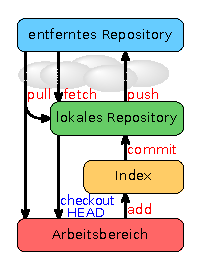
\includegraphics[scale=1.2]{git_local.eps}
				\caption{Git -- einfach erklärt}
			\end{figure}
		\end{column}
		\begin{column}{5cm}
			\begin{block}{Dezentral? Wie geht das?}
				\begin{itemize}
					\item Jeder hat das Gesamte Projekt bei sich
					\item Jede Änderung erzeugt neue eine Version
					\item Jede Version hat einen Hash als Nummer
					\item Lokal oder entfernt spielt keine Rolle!
				\end{itemize}
			\end{block}
		\end{column}
	\end{columns}
\end{frame}

\begin{frame}
	\frametitle{Git --- sicher \& stabil \hfill{} LuXeria}
	\framesubtitle{Wieso ist es sicher \& stabil?}
	\begin{block}{Sicher weil}
		\begin{itemize}
			\item Versionen sind Teil des Ganzen
			\item Nicht manipulierbar (Hash-Tree)
			\item Versionen GPG signiert
		\end{itemize}
	\end{block}
	\begin{block}{Stabil weil}
		\begin{itemize}
			\item Abgegrenzt (\lstinline$git - the stupid content tracker$)
			\item Schlank und sauber
			\item Arbeitet mit Referenzen
		\end{itemize}
	\end{block}
\end{frame}

\begin{frame}
	\frametitle{Git --- Open \& Plattformunabhängig \hfill{} LuXeria}
	\framesubtitle{Warum ist dies so wichtig?}
	\begin{block}{OpenSource}
		\begin{itemize}
			\item Freiheit
			\item Sicherheit
			\item Support
			\item Kosten
		\end{itemize}
	\end{block}
	\begin{block}{Plattformunabhängig}
		\begin{itemize}
			\item Freiheit
			\item Symbiose
			\item Flexibilität
			\item Stabilität
		\end{itemize}
	\end{block}
\end{frame}


\section{Git \& Github}
\begin{frame}
	\frametitle{}
	\tableofcontents[currentsection]
\end{frame}

\subsection{Git}
\begin{frame}
	\frametitle{Git --- Dummkopf \hfill{} LuXeria}
	\framesubtitle{Was ist Git?}
	\begin{columns}
		\begin{column}{5cm}
			\begin{figure}
				
\includegraphics[width=0.8\columnwidth]{git_logo.pdf}
				\caption{neues Git-Logo}
			\end{figure}
			\footnotesize{
			\textbf{git}[\textipa{git}] - a bastard or fool
			\epigraph{ I'm an egoistical bastard, and I name all my projects after myself.
				First Linux, now git.}{Linus Torvalds}
			}\normalsize
		\end{column}
		\begin{column}{5cm}
			\begin{block}{Überblick}
				\begin{itemize}
					\item Verwaltungssystem
					\item nicht linear
					\item dezentral
					\item sicher \& stabil
					\item OpenSource
					\item Plattformunabhängig
				\end{itemize}
			\end{block}
		\end{column}
	\end{columns}
\end{frame}

\begin{frame}
	\frametitle{Git --- nicht linear?\hfill{} LuXeria}
	\framesubtitle{Arbeiten mit Forks und Branches}
	\begin{columns}
		\begin{column}{5cm}
			\begin{figure}
				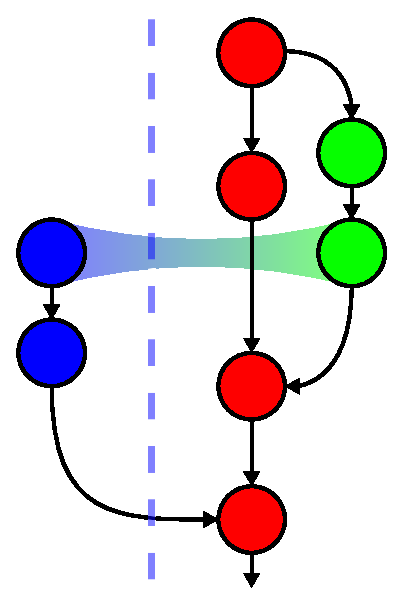
\includegraphics[scale=0.5]{git_tree.eps}\\
				\textcolor{blue}{Fork} -- \textcolor{red}{master} -- \textcolor{darkgreen}{branch}
				\caption{Projetkbaum}
			\end{figure}
		\end{column}
		\begin{column}{5cm}
			\begin{block}{Fork, Master \& Branch}
				\begin{itemize}
					\item \textcolor{red}{Arbeiten am Skript}
					\item \textcolor{darkgreen}{Version HS12}
					\item \textcolor{darkgreen}{Korrekturen im HS12}
					\item \textcolor{blue}{Studenten übernehmen Kopie und erweitern}
					\item \textcolor{red}{Das Beste kommt zusammen für FS13}
				\end{itemize}
			\end{block}
		\end{column}
	\end{columns}
\end{frame}

\begin{frame}
	\frametitle{Git --- dezentral \hfill{} LuXeria}
	\framesubtitle{Offline? Interessiert mich nicht!}
	\begin{columns}
		\begin{column}{5cm}
		\end{column}
		\begin{column}{5cm}
		\end{column}
	\end{columns}
\end{frame}



\end{document}
